\section{Gradiente Descendente}

Se trata de un algoritmo de aprendizaje iterativo clásico, basado en el método de optimización para funciones lineales de Cauchy. Haskell Curry lo estudió por primera vez para optimización no lineal en 1944 \cite{Curry1944GDNoLin}, siendo ampliamente usado a partir de las décadas de 1950-1960. Actualmente se trata de \textbf{la estrategia de entrenamiento de modelos más ampliamente usada, especialmente en los modelos de aprendizaje profundo, siendo la estrategia que mejores resultados consigue en cuanto a capacidad de generalización de los modelos y eficiencia computacional gracias a su aplicación a través del algoritmo de BP}. Como muestra de su gran adopción, en la Figura \ref{fig:mat_scopus_gd} vemos la cantidad de artículos indexados al año en la base de datos Scopus\footnote{\url{https://www.scopus.com/}}, con la siguiente búsqueda realizada a 23 de marzo de 2025:

\begin{verbatim}
	( optimization OR learning ) AND ( ( gradient AND descent ) 
	OR ( steepest AND descent ) )
\end{verbatim}





Sin embargo a nivel práctico no se usa en su versión original, sino que a lo largo del tiempo han ido surgiendo numerosas modificaciones con el objetivo de mejorar el algoritmo en diversos ámbitos: aumento de la estabilidad y la velocidad de convergencia, reducción computacional del entrenamiento, capacidad de evitar mínimos locales, etc. La literatura en este sentido es extensa, es claro que el gradiente descendente sigue siendo la mejor estrategia de optimización de parámetros de un modelo de forma general \cite{MHtrainingClase}, aunque la elección del algoritmo de optimización concreto y de su ajuste depende del problema particular que estemos tratando y generalmente se realiza de manera experimental. 


\begin{figure}[!tbp]
    \centering
    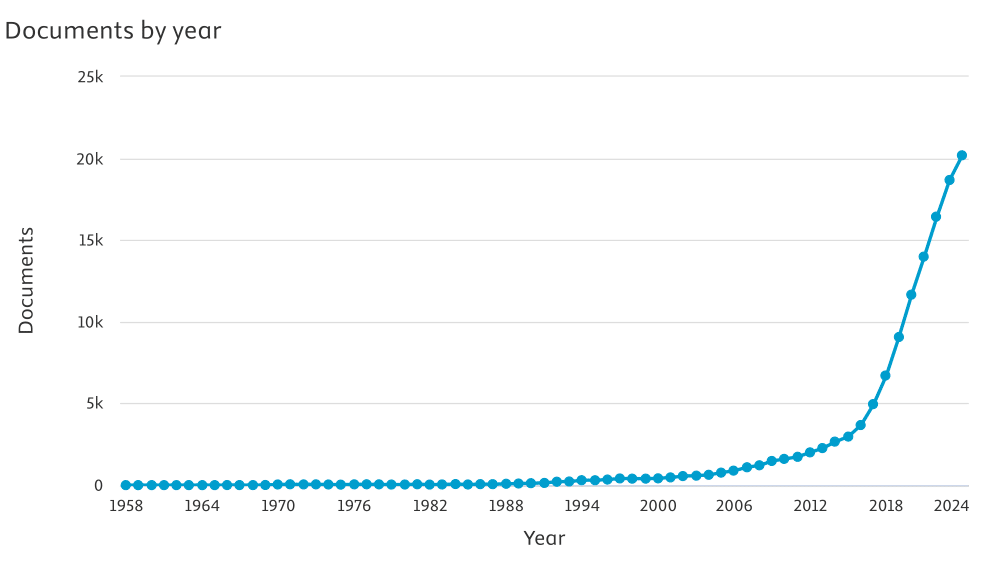
\includegraphics[width=0.75\linewidth]{Plantilla_TFG_latex//imagenes//Mat//GD/scopus_gd.png}
    \caption[Evolución del número de artículos indexados anualmente en la base de datos Scopus relacionados con optimización y aprendizaje mediante métodos de descenso de gradiente]{Evolución del número de artículos indexados anualmente en la base de datos Scopus relacionados con optimización y aprendizaje mediante métodos de descenso de gradiente. La consulta se realizó el 23 de marzo de 2025. Desde el primer registro en 1958, el total de documentos acumulados asciende a 135,000. Se observa un crecimiento exponencial en la cantidad de publicaciones a partir de aproximadamente 2010, alcanzando más de 20,000 documentos en 2024.}
    \label{fig:mat_scopus_gd}
\end{figure}

Debemos ver que \textbf{el entrenamiento de los modelos, está intrínsecamente ligado a la optimización, en concreto a la minimización de la función de coste $C$}. Este no es un problema sencillo, y como se ha mencionado antes \textbf{se trata de un problema NP-Difícil}, por tanto de existir algoritmos exactos éstos requieren demasiado coste computacional como para utilizarlos en la práctica, por lo que se buscan estrategias aproximadas como el descenso de gradiente para obtener buenas soluciones en un tiempo asequible. 

Otro factor a tener en cuenta es la generalización: no es importante únicamente obtener un error bajo en el entrenamiento sino que se mantenga cuando usamos datos de entrada nuevos, ya que nuestro objetivo es ser capaces de encontrar patrones que podamos aplicar en situaciones nuevas y no ajustar el modelo a unos datos dados.

\subsection{Gradiente descendente de Cauchy}

Procedemos a describir el método original de descenso de gradiente, propuesto en 1847 por Augustin-Louis Cauchy \cite{CauchyGD}. Es una versión más primitiva y limitada que sus desarrollos posteriores pero que nos permite obtener de forma más sencilla una visión de su funcionamiento. 

Fijamos $f:\mathbb{R}^n \rightarrow \mathbb{R}_{0}^{+}$ una función continua que no toma valores negativos. Sea $x= \left ( x_1,\ldots,x_n \right ) \in \mathbb{R}^n$. Si queremos encontrar los valores de $x_1,\ldots,x_n$ que verifican $f(x)=0$, que suponemos que existen, bastará con hacer decrecer indefinidamente los valores de la función $f$ hasta que sean muy cercanos a $0$. 

Fijamos ahora unos valores concretos $x_0 \in \mathbb{R}^n$, $u=f(x_0)$,\\ $Du= \left ( D_{x_1}u, D_{x_2}u, \ldots, D_{x_n}u \right )$ . Si tomamos $x_0'=x_0+\epsilon$ tendremos:
$$f(x_0')= f(x_0 + \epsilon) = u + \epsilon Du$$

Sea ahora $\eta >0$, tomando $\epsilon= - \eta Du$ con la fórmula anterior tenemos: 

$$f(x_0') = f(x_0 + \epsilon) = u - \eta \sum_{i=1}^{n}(D_{x_i}u)^2$$

Por tanto hemos obtenido un decremento en el valor de la función $f$ modificando los valores de sus variables en sentido contrario al gradiente, para $\eta$ suficientemente pequeño. El objetivo de la estrategia es repetir esta operación hasta que se desvanezca el valor de la función $f$.




\subsection{Gradiente descendente en el entrenamiento de modelos}

En el caso del entrenamiento de modelos la función que debemos minimizar es la función de coste $C$, que efectivamente es continua por ser composición de funciones continuas, como se verá más adelante. Como no podemos realizar un cálculo continuo para comprobar con qué valores de $\eta$ la función decrece, lo hacemos de manera iterativa, y a este $\eta$ lo llamamos ratio de aprendizaje o más comúnmente \textbf{\textit{learning rate}}. 

Si $C(W)$ es la función de coste del modelo y $W$ representa los parámetros del modelo, entonces\textbf{ la regla iterativa de actualización de los pesos en la estrategia del descenso del gradiente es la siguiente}:

\begin{equation}\label{eq:GD}
W_{t+1}=W_t - \eta \nabla C(W)
\end{equation}

En su descripción original, el gradiente se calcula usando todos los datos de entrenamiento, pero en versiones posteriores se propone dividir el conjunto de entrenamiento en varios subconjuntos disjuntos, denominados \textbf{\textit{batches}}. Cada vez que se calcula el gradiente se actualizan los pesos del modelo, y denominamos a esto una \textbf{iteración}. Cada vez que se usan todos los datos de entrenamiento para calcular el gradiente, ya sea tras una sola iteración usando todo el conjunto de entrenamiento o varias si dividimos en \textit{batches}, lo denominamos \textbf{época}.



\subsubsection{Estrategias de gradiente descendente} \label{sec:estrategias}

En base a los \textit{batches} en que dividamos el conjunto de entrenamiento tenemos varios tipos de gradiente descendente \cite{GoodFellowBook}.

\begin{itemize}
    \item \textbf{\emph{Batch Gradient Descent}} (BGD): tenemos un único \textit{batch}, cada iteración se corresponde con una época. Calculamos el gradiente usando todo el conjunto de entrenamiento. Esto ofrece un comportamiento mejor estudiado a nivel teórico, con más resultados demostrados; pero aumenta mucho el coste computacional del entrenamiento hasta el punto de que lo vuelve demasiado lento para ser usado en la práctica.

    \item \textbf{\emph{Stochastic Gradient Descent}} (SGD): Actualiza los pesos calculando el gradiente con sólo un elemento del conjunto de entrenamiento. Cada época tiene tantas iteraciones como número de elementos haya en el conjunto de entrenamiento. Esta estrategia introduce ruido en el entrenamiento ya que el gradiente se calcula de una manera aproximada, aunque esto tiene un efecto positivo ya que al provocar más irregularidad en la trayectoria de convergencia es más probable poder escapar de mínimos locales. Además es más eficiente computacionalmente que el anterior y converge más rápido en la práctica.

    \item \textbf{\emph{Mini-Batch Gradient Descent}} (MBGD): Se divide el conjunto de entrenamiento en $M$ \textit{batches} disjuntos de tamaño fijo, y se calcula el gradiente con cada \textit{batch}, por lo que habrá $M$ iteraciones en cada época. Se consigue una aproximación del gradiente con menos error al usar más datos para su cálculo y además se siguen manteniendo las propiedades que veíamos en la anterior estrategia. Es más eficiente que la anterior al conllevar menos actualizaciones de pesos. Es prácticamente la única estrategia utilizada en la realidad ya que ofrece la mayor eficiencia computacional, estabilidad y rapidez en la convergencia.
\end{itemize}

En estos dos últimos casos, \textbf{el conjunto de entrenamiento no permanece fijo}, por lo que la regla de actualización de los pesos que hemos visto en \eqref{eq:GD} quedaría de la siguiente manera:

\begin{equation}\label{eq:SGD}
	W_{t+1} = W_t - \eta \nabla C(X_{t+1}, W_t)
\end{equation}

Aunque la política para computar el gradiente sea distinta en estos 3 tipos, los englobaremos dentro de lo que denominaremos el algoritmo de gradiente descendente original, ya que existen varias modificaciones del algoritmo que aportan mejoras a través de modificar la regla de actualización de los pesos y no solo la cantidad de datos con la que se aproxima el gradiente.

\subsubsection{\textit{Learning rate}}

El parámetro $\eta$ que observamos en la ecuación \eqref{eq:GD} del gradiente descendente se denomina \textbf{\textit{learning rate}} y lo usamos para controlar la convergencia reduciendo el efecto de la magnitud del gradiente en la actualización de los parámetros. Este valor es positivo y situado en la práctica alrededor de 0.01 y 0.001 usualmente, aunque para su elección conviene realizar un análisis teórico previo o realizar pruebas prácticas (mucho más común) para elegir un valor adecuado. Este tipo de parámetros, que no son parte del modelo sino del algoritmo de aprendizaje, se denominan \textbf{hiperparámetros}. Dependiendo del tipo de algoritmo o modificación del mismo que usemos habrá diferentes hiperparámetros, siendo el \textit{learning rate} el más importante de manera general, ya que \textbf{de su valor dependerá en gran parte la convergencia del algoritmo}, pudiendo hacer que converja demasiado lento o que directamente diverja, como podemos observar en la Figura \ref{fig:lr} o en resultados sobre la convergencia en la Sección \ref{sec:convergencia}.

En cuanto a la selección de los hiperparámetros, no se enfoca como un problema donde se busque el óptimo de estos valores ya que la mayoría no son tan decisivos en la convergencia como el \textit{learning rate}, y se ofrecen valores teóricos en sus artículos de presentación que funcionan bien en casos generales. Si bien la convergencia es sensible a los valores iniciales de estos hiperparámetros que se tratan de optimizar a nivel experimental a través del ensayo y error, aunque no se realiza una búsqueda exhaustiva, invirtiéndose muchos más recursos computacionales en el entrenamiento.



\begin{figure}
    \centering
    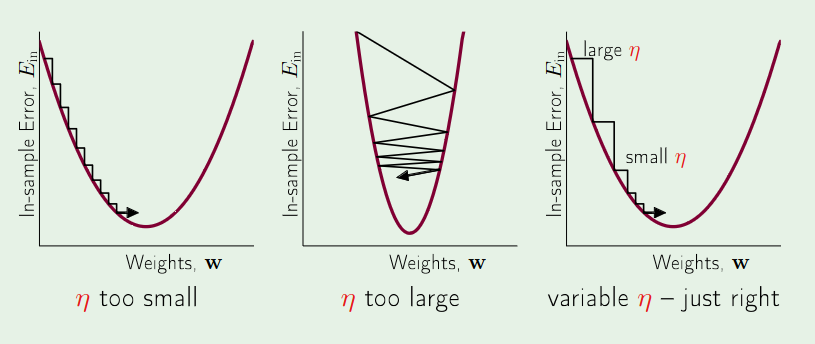
\includegraphics[width=0.75\linewidth]{Plantilla_TFG_latex//imagenes//Mat//GD/lr.png}
    \caption[Efecto del tamaño del \textit{learning rate} en el comportamiento del algoritmo de gradiente descendente]{Efecto del tamaño del \textit{learning rate} ($\eta$) en el comportamiento del algoritmo de gradiente descendente. La figura ilustra tres escenarios distintos según el valor del \textit{learning rate} ($\eta$). \textit{Izquierda}: Un valor de $\eta$ demasiado pequeño provoca una convergencia extremadamente lenta, con pasos muy cortos que tardan en alcanzar el mínimo del error de entrenamiento $E_{in}$. \textit{Centro}: Un $\eta$ demasiado grande genera oscilaciones e incluso puede impedir la convergencia, ya que los pasos del algoritmo sobrepasan el mínimo óptimo. \textit{Derecha}: Un \textit{learning rate} variable, que comienza con un valor grande y se reduce progresivamente, permite una convergencia eficiente y estable, combinando rapidez en la fase inicial y precisión cerca del óptimo. Imagen obtenida de \cite{Mostafa2012}}
    \label{fig:lr}
\end{figure}

Una táctica habitual es usar una política de \textit{learning rate} que decrezca conforme avanza el entrenamiento, de manera que el algoritmo avance con pasos más grandes cuando aún está lejos de un óptimo, con un objetivo explorador, y con pasos más pequeños cuando se va acercando, con un objetivo explotador, procurando una convergencia más estable. \cite{GoodFellowBook}. Otro enfoque común es tener un vector de \textit{learning rate} en lugar de un solo escalar, teniendo un valor para cada peso del modelo. 





\subsection{Subgradientes} \label{sec:subgrad}

Con el objetivo central de calcular el gradiente es lógico pensar que necesitamos ciertas condiciones de diferenciabilidad, aunque sean mínimas, para poder calcular el gradiente que necesitamos. Vamos a presentar el concepto de \textbf{subgradiente}, que proporciona una definición más flexible que la del gradiente y en la que nos podemos apoyar para el algoritmo de gradiente descendente.

Podemos pensar en un modelo como una composición de la suma y producto de operaciones lineales con operaciones no lineales (funciones de activación), y componiendo ésta con la función de coste del modelo obtendríamos la función $f: X \times \Omega \times Y \rightarrow \mathbb{R^+}$, que recibe los pesos del modelo, los datos de entrada y sus etiquetas correctas para proporcionar el error del modelo. Esta es la función que necesitaríamos que fuera diferenciable. Las operaciones lineales preservan la diferenciabilidad, y la composición de funciones diferenciables es diferenciable, por lo que si la función de pérdida y las funciones de activación son diferenciables, no tendremos ningún problema a la hora de calcular el gradiente.

Las funciones de coste son diferenciables de manera general, y la más común para problemas de clasificación es la entropía cruzada (o \textit{Cross Entropy}, CE, en inglés), mientras que para regresión son comunes el error cuadrático medio (ECM) y el error absoluto medio (EAM).

\begin{itemize}

    \item \textbf{ECM}: $\frac{1}{N} \sum_{i=1}^N \left (y_i - \hat{y_i} \right ) ^2$ 

    \item \textbf{EAM}: $\frac{1}{N} \sum_{i=1}^N \lvert y_i - \hat{y_i} \rvert$ 	

    \item \textbf{CE}: $  - \sum_c \hat{y}_{i,c} log(\frac{e^{y_{i,c}}}{\sum_{c'=1}^C e^{y_{i,c'}}})$
\end{itemize}

En regresión $\hat{y}_i$ es el valor real  e $y_i$ es el predicho por el modelo para el dato $i$ que será un real en ambos casos. En clasificación $\hat{y}_{i,c}$ es la etiqueta real del dato $i$ para la clase $c$, que valdrá 1 en caso de que el dato pertenezca a la clase $c$ y 0 en caso contrario, e $y_{i,c} \in [0,1]$ representa la probabilidad predicha por el modelo de que el dato $i$ pertenezca a la clase $c$. Finalmente $N$ es el número de datos y $C$ el número de clases. 


Hasta el año 2010, las funciones de activación más comunes para las capas ocultas eran la función sigmoide y la tangente hiperbólica. Estas funciones son diferenciables por lo que su uso no suponía ningún problema en la aplicación del descenso de gradiente \cite{EffBackProp}. Sobre ese año se empezó a popularizar la función de activación ReLU (\textit{Rectified Linear Unit}), gracias a su simplicidad, reducción de coste computacional y su aparición en modelos ganadores de competiciones de ImageNet como AlexNet en 2012. Desde entonces esta función, junto a algunas de sus variantes que aparecen en la Figura \ref{fig:3.ReLU} son ampliamente usadas y con buenos resultados. Sin embargo salta a la vista que esta función no es diferenciable.


\begin{figure}
    \centering
    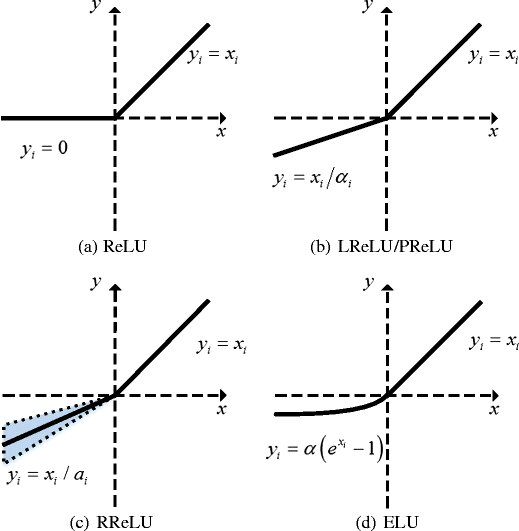
\includegraphics[width=0.5\linewidth]{3ReLU&oth.jpg}
    \caption[Funciones de activación basadas en ReLU y su impacto en la optimización mediante gradiente descendente]{Funciones de activación basadas en ReLU y su impacto en la optimización mediante gradiente descendente. La figura muestra cuatro variantes de la función de activación ReLU ($max(0,x)$), utilizadas en redes neuronales profundas para introducir no linealidad y mejorar la capacidad de representación. (a) ReLU: Mantiene valores positivos sin cambios y asigna cero a valores negativos, lo que puede causar la "neurona muerta"\footnote{El problema de la neurona muerta ocurre cuando una neurona en una red neuronal profunda deja de activarse permanentemente, es decir, su salida es siempre cero debido a valores negativos de entrada y gradientes nulos en funciones de activación como ReLU, impidiendo su actualización durante el entrenamiento} debido a gradientes nulos para $x<0$. (b) \textit{Leaky ReLU}/\textit{Parametric ReLU} (LReLU/PReLU): Introduce una pequeña pendiente controlada por un parámetro $\alpha _i$ en la región negativa para mitigar el problema de neuronas muertas. c) \textit{Randomized ReLU} (RReLU): Usa un coeficiente aleatorio $\alpha _i $ en la parte negativa durante el entrenamiento, introduciendo regularización y variabilidad en la optimización. (d) \textit{Exponential Linear Unit} (ELU): Utiliza una transformación exponencial para valores negativos, asegurando continuidad y derivabilidad en $x=0$, lo que acelera el entrenamiento y mejora la estabilidad en la actualización de pesos. Imagen obtenida de \cite{figRelu1}}
    \label{fig:3.ReLU}
\end{figure}



\textbf{Vamos a presentar entonces el concepto de subgradiente junto con algunas de sus propiedades, obtenidas de \cite{convexSubgrad}, para ver que será una extensión del gradiente (para funciones convexas) que nos permitirá usar el método de gradiente descendente con funciones que no sean diferenciables en algunos puntos pero que sí sean subdiferenciables.}

\begin{definicion}[Subgradiente]
     Sea $A \subset \mathbb{R}^n$ y $f:A \rightarrow \mathbb{R}$, $g \in \mathbb{R}^n$ es un subgradiente de $f$ en $a \in A$ si existe un entorno de $a$ $U_a$ tal que $\forall y \in U_a$ se tiene:

    $$f(a)-f(y) \leq g^T(a-y)$$
    El conjunto de los subgradientes de $f$ en $a$ se denota por $\partial f(a)$. Si existe el subgradiente de $f$ en a, decimos que $f$ es subdiferenciable en $a$.
\end{definicion}

Necesitamos también un comportamiento similar al de las funciones diferenciables, en particular necesitamos que las funciones subdiferenciables se preserven a través de las operaciones de suma, multiplicación por escalares y composición.

\begin{enumerate}

	\item{\textbf{Multiplicación escalar no negativa}: $\partial (cf) = c \cdot \partial f , c\geq0$
	
	Por definición $g$ es un subgradiente de $f$ en $x_0$ si:
	
	$$f(x) \geq f(x_0) + g^T(x-x_0), \quad  \forall x \in U_{x_0}.$$

	Multiplicando la desigualdad por $c \geq 0$:

	$$cf(x) \geq cf(x_0) + cg^T(x-x_0), \quad  \forall x \in U_{x_0}.$$

	Por tanto $cg$ es un subgradiente de $h(x)=cf(x)$ en $x_0$.

	}
	
	\item{ \textbf{Suma}: $\partial (f_1+f_2)(x) = \partial f_1(x) + \partial f_2(x)$

	Sea $g_1$ un subgradiente de $f_1$ y $g_2$ un subgradiente de $f_2$, considerando el punto $x_0 \in dom(f_1) \cap dom(f_2)$, por definición tenemos:

	$$f_1(x) \geq f_1(x_0) + g_1^T(x-x_0), \quad \forall x \in U_{x_0},$$

	$$f_2(x) \geq g_2(x_0) + g_2^T(x-x_0), \quad \forall x \in U_{x_0}.$$

	Sumamos las dos desigualdades para obtener que $g_1 + g_2$ es un subgradiente de $(f_1 + f_2)(x_0)$:

	$$f_1(x) + f_2(x) \geq f_1(x_0) + f_2(x_0) + \left ( g_1 + g_2 \right ) ^T \left ( x - x_0 \right ).$$


	}
	
	\item{ \textbf{Composición afín}: Si $h(x)=f(Mx + b) \Rightarrow \partial h(x)= M^T \partial f(Mx+b)$, donde $M \in \mathbb{R}^{m \times n}, b \in \mathbb{R}^m$.
	
	Tenemos que $g$ es un subgradiente de $f$ en $y_0=Mx_0 + b$:
	
	$$f(y) \geq f(y_0) + g^T(y-y_0), \quad \forall y \in U_{y_0}.$$

	Tomamos $y=Mx + b$ y, sustituyendo:

	$$f(Mx + b) \geq f(Mx_0 + b) + g^T(Mx + b - (Mx_0 + b))  \quad \forall x \text{ : } Mx+b \in U_{y_0},$$

	$$h(x)=f(Mx+b) \geq h(x_0) + g^TM(x-x_0) \quad forall x \text{tal que} Mx+b \in U_{y_0}.$$

	Por tanto $M^Tg$ es un subgradiente de $h(x)=f(Mx+b)$ en $x_0$.

	}
	
\end{enumerate}


Tenemos que comprobar que \textbf{el subgradiente extiende al gradiente para funciones convexas y diferenciables}, es decir, que cuando existe gradiente entonces existe un único subgradiente y coincide con él. Además hay funciones que no son diferenciables pero sí subdiferenciables. Esto último se hace evidente con el Ejemplo \ref{ej:RELUsub} de la función ReLU. Vamos a demostrar por tanto que si $f: X \subseteq \mathbb{R}^n \rightarrow \mathbb{R}^m$ es diferenciable en el punto $x\in X$ entonces  $\partial f(x)= \left \{ \nabla f(x) \right \}$. Primero recordamos algunas nociones de convexidad:


\begin{definicion}[Conjunto convexo]
    Un subconjunto $E \subseteq \mathbb{R}^n$ es convexo cuando, para cualesquiera dos puntos de $E$, el segmento que los une está contenido en $E$:

    $$x,y \in E \Rightarrow \left \{ (1-t)x + ty : t\in [0,1] \right \} \subset E.$$
\end{definicion}




\begin{definicion}[Función convexa]
    Sea $E \subset \mathbb{R}^n$ un conjunto convexo no vacío y sea $f:E \rightarrow \mathbb{R}$, $f$ es una función convexa en $E$ si, y solo si:

    $$f( (1-t)y + tx) \leq (1-t) f(y) + tf(x), \quad \forall t \in [0,1], \forall x,y \in E.$$
\end{definicion}

Cuando $f$ es convexa y diferenciable en un entorno $U_x$ de $x$ el gradiente satiface 

$$  f(y) = f(x) + \nabla f(x)^T(y-x) + o(\|y-x \|) \quad \forall y \in U_x .$$

Por tanto tenemos

$$ f(y) \geq f(x) + \nabla f(x)^T(y-x) \quad \forall y \in U_x.$$

Es decir que el gradiente de $f$ en $x$ es también un subgradiente de $f$ en $x$. Tenemos que $\nabla f(x) \in \partial f(x)$, nos queda demostrar que es único. Para ello vamos a suponer que existe otro subgradiente de $f$ en $x$, $g \in \partial f(x)$. Sea $u=x+tw$, definimos la función

$$\phi(t)=f(u)-f(x)- g^T(u-x) = f(x+tw) -f(x) - g^T(tw) \geq 0,$$

donde se ha usado que $g \in \partial f(x)$ para ver que es no negativa. Derivamos la función para obtener $\phi'(t) = \nabla f(x)^Tw - g^Tw$. Vemos que para $t=0$ se tiene que $\phi(0)=0$, con lo que hay un mínimo en ese punto. Tenemos por tanto que $\phi'(0)=0$ o equivalentemente $\nabla f(x)^Tw=g^Tw$. Como $w$ es arbitrario, concluimos que $g=\nabla f(x)$. Como el gradiente es un subgradiente, y todo subgradiente coincide con él, se tiene que es el único subgradiente de $f$ en $x$, $\partial f(x) = \left \{ \nabla f(x) \right \}$. 



Ahora vamos a ver cómo se relacionan los subgradientes y las funciones convexas que no necesariamente sean diferenciables.



\begin{proposicion}[Existencia de subgradientes]
\label{prop:subgrad}
    Sea $E \subset \mathbb{R}^n$ un conjunto convexo y $f:E \rightarrow \mathbb{R}$. Si $\forall x \in E, \partial f(x) \neq \emptyset$ entonces $f$ es una función convexa. Recíprocamente, si $f$ es convexa  entonces se tiene que $\forall x \in int(E)$ $\partial f(x) \neq \emptyset$.
\end{proposicion}

Esta proposición nos asegura que \textbf{las funciones convexas siempre tienen subgradiente en su interior}, en particular las funciones de activación convexas como es el caso de la función ReLU. Para demostrarla, primero vamos a necesitar de un teorema en el ámbito de la convexidad:

\begin{teorema}[Teorema del Hiperplano de apoyo]
    Sea $E \subset \mathbb{R}^n$ un conjunto convexo y $x_0 \in Fr(E)$ un puntro de la frontera de $E$. Entonces, $\exists w \in \mathbb{R}^n, w \neq 0$ tal que
    $$\forall x \in E, \quad w^Tx \geq w^T x_0.$$
\end{teorema}

\vspace{1cm}


\begin{flushleft}
   \textbf{\textit{Demostración de la Proposición \ref{prop:subgrad}.}}
\end{flushleft} 
Para la primera implicación, queremos probar que si para todo punto $x \in E$ existe al menos un subgradiente de $f(x)$ entonces se verifica
$$f((1-t)x+ty) \leq (1-x)f(x)+tf(y) \quad \forall x,y \in E, t \in [0,1],$$
es decir, que $f$ es convexa. Tomamos $g \in \partial(z),$ $z \in E$ ya que $\forall z \in E,  \partial f(z) \neq \emptyset $ , y tenemos por la definición de subgradiente:

\begin{align}
	f(z) - f(x) \leq g^T(z-x), \notag \\
	f(z) - f(y) \leq g^T(z-y), \label{eq:des2}
\end{align}

para $x,y \in E$. Tomamos $z=(1-t)x + ty$ y sustituimos:

\begin{align}	
	f((1-t)x + ty) - f(x) &\leq g^T(((1-t)x + ty)-x), \notag \\
	f((1-t)x + ty) + g^T(x - ((1-t)x-ty)) &\leq f(x), \notag \\
	f((1-t)x + ty) + g^T(t(x-y)) &\leq f(x), \notag \\
	f((1-t)x + ty) + tg^T(x-y) &\leq f(x). \label{proof1:f(x)}
\end{align}


Desarrollando en \eqref{eq:des2} de manera análoga obtenemos

\begin{equation}\label{proof1:f(y)}
    f((1-t)x + ty) + (1-t)g^T(y-x)) \leq f(y).
\end{equation}

Ahora multiplicamos la desigualdad \eqref{proof1:f(x)} por $(1-t)$ y la \eqref{proof1:f(y)} por $t$, y de su suma obtenemos:

\begin{align*}
	(1-t)f(x) + tf(y) &\geq  (1-t)f((1-t)x+ty) + t(1-t)g^T(x-y) \\
	&+ tf((1-t)x+ty) + t(1-t)g^T(y-x) \\
	 &= f((1-t)x + ty) + t(1-t) g^T(x-y) + t(1-t)g^T(y-x) \\
	&= f((1-t)x+ty)
\end{align*}

donde se ha usado que $g^T(x-y) + g^T(y-x)=0$. Entonces tenemos que $(1-t)f(x) + tf(y) \geq f((1-t)x + ty), $ $ \forall x,y \in E, $ $ t \in [0,1]$. Por tanto $f$ es convexa, como queríamos probar.

Ahora vamos a probar que $f$ tiene algún subgradiente en $int(E)$ si es convexa. Definimos el epigrafo de una función $f$ como

 $$epi(f)=\left \{ (x,t) \in E \times \mathbb{R} : t \geq f(x) \right \}.$$

Es obvio que f es convexa si y sólo si su epigrafo es un conjunto convexo. Vamos a aprovechar esta propiedad y vamos a construir un subgradiente usando un hiperplano de apoyo al epigrafo de la función. Sea $x \in E$, claramente $(x, f(x)) \in Fr(epi(f))$, y $epi(f)$ es un conjunto convexo por ser $f$ convexa. Entonces usando el Teorema del Hiperplano de Apoyo, existe $(a,b) \in \mathbb{R}^n \times \mathbb{R}$ tal que

\begin{equation}\label{proof1:epi}
    a^Tx + bf(x) \geq a^Ty + bt, \quad \forall (y,t) \in epi(f).
\end{equation}

Reordenando tenemos

$$b(f(x)-t) \geq a^Ty - a^Tx.$$

Como $t \in [f(x), + \infty [$, para que se mantenga la igualdad incluso cuando $t \rightarrow \infty$, debe ocurrir que $b\leq 0$. Ahora vamos a asumir que $x \in int(E)$. Entonces tomamos $\epsilon > 0$, verificando que $y=x+\epsilon a \in E$, lo que implica que $b\neq 0$, ya que si $b=0$ entonces necesariamente $a=0$. Reescribiendo \eqref{proof1:epi} con $t=f(y)$ obtenemos

$$f(x) - f(y) \leq \frac{1}{|b|} a^T (x-y).$$

Por tanto $\frac{a}{|b|} \in \partial f(x)$, lo que demuestra la otra parte de la implicación.

\begin{comment}
	
	Para la última parte, sea $f$ una función convexa y diferenciable. Entonces por definición de convexidad para $t \in [0,1]$ y $x,y \in E$ tenemos
	
	$$tf(y) + (1-t)f(x) \geq f((1-t)x + ty).$$
	
	Deducimos entonces que
	
	\begin{align*}
		f(y) &\geq \frac{f((1-t)x + ty) - (1-t)f(x)}{t}
		
		&= f(x) + \frac{f(x + t(y-x)) - f(x)}{t}
	
		&\xrightarrow[t \rightarrow 0]{} \quad f(x) + \nabla f(x)^T (y-x).
	\end{align*}
	
	
	
	Lo que demuestra que $\nabla f(x) \in \partial f(x)$.
\end{comment}


\begin{flushright}
    $\square$
\end{flushright} 





\textbf{Tenemos entonces que el subgradiente es una extensión del gradiente para funciones convexas en aquellos puntos que no son diferenciables}. Por ello podríamos decir que existe el método de descenso de subgradiente, que permite usar funciones que no son diferenciables en todos los puntos, y que se usa de manera implícita en el momento en el que en un modelo se usan funciones de la familia ReLU. Conviene destacar esta diferencia para no perder la rigurosidad, aunque solo sea una formalidad, ya que realmente no se hacen diferencias entre uno y otro método, así que nos seguiremos refiriendo al método de descenso de gradiente aunque estemos trabajando con subgradientes. \textbf{En la práctica simplemente se elige un valor predeterminado para la derivada en el punto que estas funciones no son diferenciables}.

\begin{ejemplo}[Subgradiente de la función ReLU]\label{ej:RELUsub}
     La función ReLU es continua en todo el dominio y diferenciable en $]-\infty,0[ \cup ]0,\infty[$. Su subgradiente es el siguiente:

    $$ \nabla ReLU(x)=\left\{\begin{matrix}
1 \quad si \quad x \in ]0,\infty[ \\
c \in [0,1] \quad si \quad x=0\\
0 \quad si \quad x \in ]-\infty,0[
\end{matrix}\right.$$
\end{ejemplo}

En \cite{ReLuat0} se analiza la \textbf{elección del valor que toma el subgradiente} en el punto $x=0$ y se analiza su influencia en el entrenamiento de modelos. Se discuten varios valores y se observa que \textbf{el 0 es el que mejor resultados ofrece} en cuanto al rendimiento de los modelos entrenados.




\subsection{Convergencia} \label{sec:convergencia}

\textbf{La convergencia es un aspecto fundamental en el algoritmo de gradiente descendente}. Dado que se trata de un método de optimización iterativo, su objetivo es aproximarse al mínimo global de la función de coste a lo largo de sucesivas iteraciones o, en su defecto, alcanzar un mínimo local que proporcione una solución subóptima. El algoritmo actualiza los parámetros en dirección opuesta al gradiente, por lo que, en caso de converger, lo hará hacia puntos donde el gradiente se aproxima a cero. Dos factores clave en el análisis de su convergencia son la variante del algoritmo utilizada (estocástica o determinista) y la convexidad de la función de coste.


Los estudios teóricos sobre la convergencia del algoritmo de descenso del gradiente son numerosos y diversos \cite{optimal_gd, de2015global, mertikopoulos2020almost, fehrman2020convergence, tibshirani2013convex}. Sin embargo, su aplicabilidad práctica es limitada, ya que suelen basarse en hipótesis demasiado estrictas sobre la función de coste, las cuales rara vez se cumplen en problemas reales o resultan demasiado costosas de verificar. A pesar de estas limitaciones, dichos desarrollos contribuyen al avance hacia una teoría más aplicable en la práctica, lo que resalta la importancia de comprender sus fundamentos y proponer mejoras. Los principales desafíos para establecer un marco teórico con aplicaciones prácticas son:

\begin{itemize}

    \item No existen resultados generales que nos permitan conocer el comportamiento de la convergencia del algoritmo en el problema que estemos tratando con un coste computacional asequible. Los resultados son muy específicos y dependen de la función de coste, el valor de los hiperparámetros y la versión del algoritmo de gradiente descendente que estemos utilizando.

    \item El estudio teórico de la función de coste es muy complejo y requiere muchos recursos computacionales. Por lo tanto, la tendencia a nivel experimental es invertir esos recursos en el entrenamiento, ya que ofrece mejores resultados en relación coste/beneficio de manera general que el estudio teórico de los elementos del algoritmo. Además, es un procedimiento genérico aplicable en cualquier problema, por lo que resulta más sencillo.

   
\end{itemize}



\subsubsection{Convergencia para \textit{Batch Gradient Descent}}

La convergencia de la versión BGD es menos compleja que en las versiones por \textit{batches}, ya que se emplea la totalidad del conjunto de entrenamiento para calcular el gradiente en cada iteración. A diferencia de las versiones SGD y MBGD, aquí no introducimos ruido estocástico por la aproximación de éste cálculo, por lo que al no haber variabilidad en la estimación del gradiente no se requiere de herramientas de análisis probabilístico. Como resultado, \textbf{el estudio de la convergencia de BGD puede abordarse principalmente desde un enfoque determinista, simplificando el tratamiento teórico con respecto a sus versiones estocásticas}.

\textbf{Analizaremos el caso en que la función de coste sea convexa}. En esta situación, probablemente sólo existirá un punto crítico\footnote{Si existiera una región donde la función fuera constante, cada punto de la región sería un punto crítico pero esto sería extraordinariamente extraño.} y será un mínimo global, por lo que no es necesario preocuparse por la posibilidad de que el algoritmo se estanque en un mínimo local, ya que, si converge, alcanzará la solución óptima. Además, \textbf{el análisis de la convergencia en este contexto es considerablemente más accesible, lo que ha permitido el desarrollo de resultados teóricos más sólidos y abundantes en comparación con el caso no convexo}. No obstante, en la práctica, la función de coste rara vez es convexa \cite{LiVisualizing}, y verificar su convexidad es un problema NP-Difícil \cite{Ahmadi_2011_NP_Convex}. Por esta razón, generalmente no se realiza un análisis teórico previo sobre la función ni sobre la convergencia antes de entrenar el modelo.



Antes de enunciar el Teorema \ref{proof:gdconvex}, presentaremos un resultado fundamental para su demostración. Demostraremos esta proposición, ya que, si bien es sencilla, no es trivial.


\begin{proposicion}\label{prop:hess}
	Sea $f: \mathbb{R}^n \rightarrow \mathbb{R}$ de clase $C^2$ y convexa, con gradiente globalmente Lipschitz continuo con constante $L$. Entonces la matriz Hessiana de $f$ está mayorada por $LI$ en el sentido semidefinido positivo, es decir, se tiene que para todo $v \in \mathbb{R}^n$

\begin{equation*} 
	v^T\nabla ^2f(x)v \leq Lv^Tv = L \|v \|^2.
\end{equation*}

Equivalentemente, se tiene que todos los autovalores de $\nabla ^2f(x)$ están mayorados por $L$. Usaremos la notación $\nabla ^2 f(x) \preceq LI$.
\end{proposicion}


\vspace{1cm}
\begin{flushleft}
   \textbf{\textit{Demostración.}}
\end{flushleft} 

Por definición, la continuidad Lipschitz global del gradiente implica que para cualquier $x,y \in \mathbb{R}^n$,

\begin{equation*} 
	\| \nabla f(y) - \nabla f(x) \| \leq L \| y - x \|.
\end{equation*}

Consideramos un vector unitario $v \in \mathbb{R}^n$ y un real $t>0$. Para $y=x + tv$, la condición de Lipschitz nos da:

\begin{equation*} 
	\| \nabla f (x+tv) - \nabla f(x) \| \leq L \| tv\| = Lt.	
\end{equation*}

Dividiendo en ambos lados por $t$ y tomando el límite cuando $t \rightarrow 0$ obtenemos que

\begin{equation}\label{eq:acotporL}
	\| \nabla ^2 f(x) v \| \leq L.
\end{equation}

Por otro lado, como la matriz Hessiana está bien definida por ser $f$ de clase $C^2$, entonces es simétrica. Ello implica que todos sus autovalores $\lambda _i$ son reales, y que su norma es igual al radio espectral, es decir,

\begin{equation*}
	\| \nabla ^2 f(x) \| = \rho(\nabla ^2 f(x)) = \text{máx}\left \{ | \lambda_i | \right \}.
\end{equation*}

Utilizando que $f$ es convexa, sabemos que su matriz Hessiana es semidefinida positiva, lo que implica que todos sus autovalores son no negativos, y por tanto de la ecuación anterior obtenemos que 

\begin{equation*}
	\| \nabla ^2 f(x) \| = \rho(\nabla ^2 f(x)) = \text{máx}\left \{ \lambda_i \right \}.
\end{equation*}

Como $\| \nabla ^2 f(x) v \| \leq L$ para cualquier vector unitario $v$, utilizando la igualdad anterior y la desigualdad \eqref{eq:acotporL} se tiene que 

\begin{equation*}
	\text{máx}\left \{ \lambda_i \right \} = \| \nabla ^2 f(x) \| = \underset{\|v| \| =1}{\text{sup}} \| \nabla ^2 f(x) v \| \leq L.
\end{equation*}

Por tanto concluimos que todo autovalor de $\nabla ^2 f(x)$ está mayorado por $L$, y entonces $\nabla ^2 f(x) \preceq LI$.

\begin{flushright}
    $\square$
\end{flushright} 

\begin{observacion}
	Es importante la globalidad de la continuidad Lipschitz del gradiente. Podemos pensar en la función $f(x)=x^4$, que es de clase $C^2$, convexa y su gradiente es localmente Lipschitz continuo en cualquier intervalo $[ -M,M ]$, con constante de Lipschitz $12M^2$. Sin embargo $\nabla f(x)$ no es globalmente Lipschitz continuo, ya que $f''(x)=12x^2$ no está acotada en $\mathbb{R}$. Por tanto no se verifica la desigualdad de la proposición anterior.
\end{observacion}




Ahora sí ya estamos en condiciones de enunciar y demostrar el siguiente teorema clave:

\begin{teorema}[Convergencia para BGD]\label{proof:gdconvex}
    Suponemos la función $f: \mathbb{R}^n \rightarrow \mathbb{R}$ de clase $C^2$ y convexa, con gradiente globalmente Lipschitz continuo con constante $L>0$, $\| \nabla f(x) - \nabla f(y) \|_2 \leq L \|x-y\|_2 \quad \forall x, y \in \mathbb{R}^n$. Si ejecutamos el algoritmo de gradiente descendente $k$ iteraciones con un $\eta<1/L$ constante, el error disminuirá tras cada iteración, llegando a una solución $x^{(k)}$ que satisface la siguiente desigualdad:

    $$f(x^{(k)})-f(x^*) \leq \frac{\|x^{(0)}-x^* \|^2_2}{2\eta k}$$

    donde $x^*$ es el mínimo global de la función de error. Es decir, $x^{(k)}$ representa los pesos del modelo en la iteración $k$ y $x^*$ es el conjunto de parámetros que minimiza la función de error.
\end{teorema}

\vspace{1cm}

\begin{flushleft}
   \textbf{\textit{Demostración.}}
\end{flushleft} 

Suponemos que el conjunto de datos con el que entrenamos es constante, por lo tanto el error del modelo, $f(x)$, sólo dependerá de los parámetros $x$. Partimos de una función $f: \mathbb{R}^n \rightarrow \mathbb{R}$ que cumple las hipótesis del teorema. 

Al ser $f \in C^2$, usamos la expansión de Taylor de segundo orden alrededor de $x$: 

\begin{equation*}
	f(y) = f(x) + \nabla f(x)^T (y-x) + \frac{1}{2} (y-x)^T \nabla^2 f(x) (y-x) 
\end{equation*}

Como $f$ cumple las condiciones de la Proposición \ref{prop:hess} entonces se tiene

\begin{equation*} 
	(y-x)^T\nabla ^2f(x)(y-x) \leq Lv^Tv = L \|y-x \|^2.
\end{equation*}

Y por tanto:

\begin{equation*}
    f(y) \leq f(x) + \nabla f(x)^T(y-x) + \frac{1}{2}L \|y - x \|^2_2.
\end{equation*}

Consideramos ahora $y$ como la actualización de los pesos del gradiente descendente, $y=x - \eta \nabla f(x)=x^+$. 


\begin{align*}
    f(x^+) &\leq f(x) + \nabla f(x)^T(x^+-x) + \frac{1}{2}L \|x^+ - x \|^2_2 \\
    &= f(x) + \nabla f(x)^T(x - \eta \nabla f(x) -x) + \frac{1}{2}L \|x - \eta \nabla f(x) - x \|^2_2 \\
    &= f(x) - \eta \nabla f(x)^T \nabla f(x) + \frac{1}{2} L \| \eta \nabla f(x) \|^2_2 \\
    &= f(x) - \eta \| \nabla f(x) \|^2_2 + \frac{1}{2} L \eta^2 \| \nabla f(x) \|^2_2 \\
    &= f(x) - (1- \frac{1}{2}L \eta) \eta \| \nabla f(x) \|^2_2.
\end{align*}

Usamos $\eta \leq \frac{1}{L}$ para ver que $-(1-\frac{1}{2}L \eta)= \frac{1}{2} L \eta - 1 \leq \frac{1}{2} L (\frac{1}{L}) - 1 = -\frac{1}{2}$, y sustituyendo esta expresión en la desigualdad anterior obtenemos 

\begin{equation}\label{eq:gdproof1}
	f(x^+) \leq f(x) - \frac{1}{2} \eta \| \nabla f(x) \|^2_2 .
\end{equation}

Esta última desigualdad se traduce en que tras cada iteración del algoritmo del descenso de gradiente el valor del error del modelo es estrictamente decreciente, ya que el valor de $\frac{1}{2} \eta \| \nabla f(x) \|^2_2$ siempre es mayor que 0 a no ser que $\nabla f(x)=0$, en cuyo caso habremos encontrado el óptimo. 

Ahora vamos a acotar el valor del error en la siguiente iteración, $f(x^+)$, en términos del valor óptimo de error $f(x^*)$. Como $f$ es una función convexa se tiene

\begin{align*}
    f(x) &\leq f(x^*) + \nabla f(x)^T (x-x^*).
\end{align*}

Sustituyendo en \eqref{eq:gdproof1} obtenemos

\begin{align*}
    f(x^+) &\leq f(x^*) + \nabla f(x)^T (x-x^*) - \frac{\eta}{2} \| \nabla f(x) \| ^2_2 \\ 
    f(x^+) - f(x^*) &\leq  \frac{1}{2\eta}  \left ( 2 \eta \nabla f(x)^T (x-x^*) - \eta ^2 \| \nabla f(x) \| ^2_2 \right ) \\ 
    f(x^+) - f(x^*) &\leq  \frac{1}{2\eta}  \left ( 2 \eta \nabla f(x)^T (x-x^*) - \eta ^2 \| \nabla f(x) \| ^2_2 - \| x - x^* \|^2_2 + \| x - x^* \|^2_2 \right ).    
\end{align*}

Como $  2 \eta \nabla f(x)^T (x-x^*) - \eta ^2 \| \nabla f(x) \| ^2_2 - \| x - x^* \|^2_2 = \| x - \eta \nabla f(x) - x^* \|^2_2 $, se tiene que

$$ f(x^+) - f(x^*) \leq  \frac{1}{2\eta}  \left ( \| x - x^* \|^2_2 -  \| x - \eta \nabla f(x) - x^* \|^2_2 \right ) .$$

Usamos ahora la definición de $x^+$ en esta última desigualdad

$$ f(x^+) - f(x^*) \leq  \frac{1}{2\eta}  \left ( \| x - x^* \|^2_2 -  \| x^+ - x^* \|^2_2 \right ) .$$

Hacemos la sumatoria sobre las $k$ primeras iteraciones y tenemos

\begin{align*}
    \sum^k_{i=1} \left ( f(x^{(i)}) - f(x^*) \right ) &\leq \sum^k_{i=1} \frac{1}{2\eta}  \left ( \| x^{(i-1)} - x^* \|^2_2 -  \| x^{(i)} - x^* \|^2_2 \right ) \\ 
    &=\frac{1}{2\eta}  \left ( \| x^{(0)} - x^* \|^2_2 -  \| x^{(k)} - x^* \|^2_2 \right ) \\ 
    &\leq \frac{1}{2\eta}  \left ( \| x^{(0)} - x^* \|^2_2 \right ). 
\end{align*}

El sumatorio de la derecha ha desaparecido ya que es una suma telescópica. Usando que $f$ decrece con cada iteración, e introduciendo la anterior desigualdad, finalmente llegamos a donde queríamos:

$$f(x^{(k)}) - f(x^*) \leq \frac{1}{k} \sum ^k _{i=1} \left ( f(x^{(i)}) - f(x^*) \right ) \leq \frac{\|x^{(0)}-x^* \|^2_2}{2\eta k} .$$


\begin{flushright}
    $\square$
\end{flushright} 


Este teorema garantiza que, \textbf{bajo las condiciones establecidas, el algoritmo BGD converge con una tasa de convergencia de $O(1/k)$}. Se trata de un resultado teórico sólido; sin embargo, su aplicabilidad en la práctica es limitada en la mayoría de los casos. En primer lugar, el cálculo exacto de la constante de Lipschitz $L$ es computacionalmente costoso, por lo que el valor de $\eta$ suele determinarse mediante aproximaciones experimentales.



\subsubsection{Convergencia para versiones estocásticas}


Podemos obtener un resultado mucho más práctico para versiones estocásticas del algoritmo (recordamos que en la práctica MBGD es la única versión utilizada). Dicho resultado será un poco más débil que el anterior, ya que solo aseguraremos converger a un mínimo local, pero podremos relajar ciertas condiciones de diferenciabilidad y suavidad. A partir de ahora usaremos SGD para referirnos de manera general a las versiones estocásticas del algoritmo de gradiente descendente, tanto SGD como MBGD. Usando la teoría de algoritmos aproximados estocásticos, con el teorema de Robbins-Siegmund tenemos que bajo las siguientes condiciones, cuando la función es convexa se tiene la convergencia casi segura al mínimo global y cuando no lo es hay convergencia casi segura a un mínimo local. Esto nos da un criterio sencillo con el que aseguramos la convergencia, y que no depende de parámetros como la constante de Lipschitz que son complejos de computar.

Usamos como referencia el libro \cite{stochastic}. En primer lugar, vamos a introducir los conceptos de martingala, supermartingala y casi supermartingala, que son tipos de procesos estocásticos. Luego enunciaremos un teorema, el de Robbins-Siegmund, que proporciona un fuerte resultado de convergencia para los procesos casi supermartingalas. Demostrando que el algoritmo de SGD es un proceso de este tipo precisamente, enunciaremos el teorema de convergencia para estos algoritmos, demostrándolo en gran parte gracias al teorema de Robbins-Siegmund.





Vamos a hacer la notación un poco más compacta. Si $X_1, X_2, \ldots$ es una sucesión de variables aleatorias usaremos $\mathcal{F}_n$ para denotar ``la información contenida en $X_1, \ldots, X_n$". Usamos $E[Y | \mathcal{F}_n]$ en lugar de $E[Y | X_1, \ldots, X_n]$.

Una \textbf{martingala} es un modelo de juego justo, que en términos de procesos estocásticos se refiere a \textbf{una situación donde el valor esperado de ganancias de un jugador, dada toda la información pasada, permanece inalterado a lo largo del tiempo}. Si $X_n$ representa la riqueza de un jugador en el momento $n$, el juego se considera justo si $E[X_{n+1} | X_1, X_2, \ldots, X_{n-1}, X_n] = X_n \quad \forall n$, lo que significa que la riqueza futura esperada es igual a la riqueza presente, dado todo el historial previo. Esto implica que no hay una estrategia sistemática para ganar o perder dinero con el tiempo basándose solo en los resultados pasados.

Denotamos por $\left \{ \mathcal{F}_n \right \}$ una sucesión creciente de información, es decir, para cada $n$ tenemos una sucesión de variables aleatorias $\mathcal{A}_n$ tal que $\mathcal{A}_m \subseteq \mathcal{A}_n$ si $m<n$. La información que tenemos en el momento $n$ es el valor de todas las variables en $\mathcal{A}_n$. La suposición $\mathcal{A}_m \subseteq \mathcal{A}_n$ implica que no perdemos información. Decimos que una variable aleatoria $X$ es $\mathcal{F}_n$-medible si podemos determinar el valor de $X$ en caso de conocer el valor de todas las variables aleatorias en $\mathcal{A}_n$. A menudo está sucesión creciente de información $\mathcal{F}_n$ se denomina filtración.

\textbf{Decimos que una sucesión de variables aleatorias $M_0, M_1, M_2, \ldots$ con $E[ |M_i|] < \infty$ es una martingala con respecto a $\left \{ \mathcal{F} \right \} _n$ si cada $M_n$ es medible con respecto a $\mathcal{F}_n$ y para cada $m<n$,}

\begin{equation}\label{eq:martingala}
	E[M_n | \mathcal{F}_m] = M_n,
\end{equation}

o equivalentemente,

\begin{equation}
	E[M_n - M_m |\mathcal{F}_m] = 0.
\end{equation}	

La condición $E[|M_i|] < \infty$ es necesaria para garantizar que las esperanzas condicionadas están bien definidas. Si $\mathcal{F}_n$ es la información en variables aleatorias $X_1, \ldots, X_n$ entonces también diremos que $M_0, M_1, \ldots$ es una martingala con respecto a $X_0, X_1, \ldots$. A veces diremos que $M_0, M_1, \ldots$ es una martingala sin hacer referencia a la filtración $\mathcal{F}_n$. En ese caso significará que la sucesión $M_n$ es una martingala con respecto a sí misma. 

\textbf{Un proceso $M_n$ con $E[|M_n|] < \infty$ es una supermartingala con respecto a $\left \{ \mathcal{F}_n \right \}$ si para cada $m<n$ se tiene $E[M_n | \mathcal{F}_m] \leq M_m$}. En otras palabras, una supermartingala es un juego injusto. Si un proceso estocástico no verifica la desigualdad anterior, pero verifica que 

\begin{equation*}
	E[M_n | \mathcal{F}_m] \leq (1 + \beta _m ) M_m + \xi _m - \zeta _m
\end{equation*}

para $m<n$ y $\beta _n, \xi _n, \zeta _n \geq 0$ siendo $\mathcal{F}_n$-medibles, \textbf{decimos entonces que $M_n$ es una casi supermartingala}, y la denominaremos  no negativa si $M_n>0 \quad \forall n$. El Teorema de Robbins-Siegmund es un resultado clave para la demostración de la convergencia de las versiones estocásticas del gradiente descendente que enunciaremos a continuación. Primero vamos a enunciar el Teorema de Doob sobre la convergencia de supermartingalas, herramienta clave en la teoría de martingalas.


\begin{teorema}[Teorema de Convergencia de Supermartingalas]\label{teor:convdoob}
 Si $V_n$ es una supermartingala y está acotada inferiormente casi seguramente, entonces $V_n$ converge casi seguro a una variable aleatoria integrable $V_{\infty}$.
 \end{teorema}






Ahora sí, enunciamos y demostramos el teorema de Robbins-Siegmund, que es un \textbf{poderoso resultado de convergencia para procesos estocásticos no negativos que son casi supermartingalas}. 

\begin{teorema}[Teorema de Robbins-Siegmund]\label{teor:sig}
	Suponemos que $V_n$ es una casi supermartingala no negativa. Si 

	$$ \sum_{n=1}^{\infty} \beta_n < \infty \quad \text{y} \quad \sum_{n=1}^{\infty} \xi_n < \infty \quad \text{casi seguro,}$$

	entonces existe una variable aleatoria no negativa $V_{\infty}$ que verifica

	$$ \displaystyle \lim_{n \to \infty}V_n = V_{\infty} \quad \text{y} \quad \sum_{n=1}^{\infty} \zeta < \infty \quad \text{casi seguro.}$$
\end{teorema}


\begin{flushleft}
   \textbf{\textit{Demostración.}}
\end{flushleft} 

Dada $V_n$ una casi supermartingala no negativa, vamos a construir una supermartingala auxiliar a partir de ella y aplicarle el Teorema de Convergencia de Supermartingalas para ver que converge, y posteriormente demostramos que la convergencia de la casi supermartingala está relacionada con la convergencia de nuestra supermartingala auxiliar. Por definición $V_n$ es un proceso estocástico no negativo que verifica la desigualdad

\begin{equation}\label{eq:rb_eq1}
	E[V_n | \mathcal{F}_m] \leq (1 + \beta _m ) V_m + \xi _m - \zeta _m
\end{equation}

para $m<n$ y $\beta _n, \xi _n, \zeta _n \geq 0$ siendo $\mathcal{F}_n$-medibles. A partir de $V_n$ definimos un proceso auxiliar supermartingala $W_n$, como


\begin{equation*}
	W_n = V_n + \sum_{k=1}^{n-1} \zeta_k - \sum_{k=1}^{n-1} (\beta_k + \xi_k).
\end{equation*}

Ahora vamos a verificar que $W_n$ es una supermartingala calculando su esperanza condicionada:

\begin{align*}
E[W_{n+1} \mid \mathcal{F}_n] 
&= E\left[V_{n+1} + \sum_{k=1}^n \zeta_k - \sum_{k=1}^n (\beta_k + \xi_k) \mid \mathcal{F}_n\right] \\
&= E[V_{n+1} \mid \mathcal{F}_n] + \sum_{k=1}^n \zeta_k - \sum_{k=1}^n (\beta_k + \xi_k).
\end{align*}

Como $V_n$ es por hipótesis una casi supermartingala, usamos la desigualdad \eqref{eq:rb_eq1} en la ecuación anterior, y simplificando obtenemos:

\begin{align*}
E[W_{n+1} \mid \mathcal{F}_n] \leq& V_n + \beta_n - \zeta_n + \xi_n + \sum_{k=1}^n \zeta_k - \sum_{k=1}^n (\beta_k + \xi_k) \\
=& V_n + \sum_{k=1}^{n-1} \zeta_k - \sum_{k=1}^{n-1} (\beta_k + \xi_k) = W_n.
\end{align*}

Y por tanto $W_n$ es una supermartingala. Ahora vamos a comprobar que está acotada inferiormente para poder aplicar el Teorema \ref{teor:convdoob}. Como por definición $V_n \geq 0$ y $\sum_{k=1}^{n-1} \zeta_k \geq 0$, tenemos que $W_n \geq -\sum_{k=1}^{n-1} (\beta_k + \xi_k)$. Por la hipótesis del Teorema $\sum_{k=1}^\infty (\beta_k + \xi_k) < \infty$ casi seguro, por lo que la cota inferior $-\sum_{k=1}^{n-1} (\beta_k + \xi_k)$ es finita casi seguro. Podemos ahora aplicar el Teorema de Convergencia de Supermartingalas para afirmar que $W_n$ converge casi seguro a $W_{\infty}$.

Como $W_n$ converge casi seguro y $\sum_{k=1}^{n-1} (\beta_k + \xi_k) < \infty$ casi seguro, de la definición de $W_n$ tenemos que 

 

\begin{equation*}
V_n + \sum_{k=1}^{n-1} \zeta_k = W_n + \sum_{k=1}^{n-1} (\beta_k + \xi_k)
\end{equation*}

y que los dos términos del lado derecho convergen casi seguro. Eso significa que $V_n + \sum_{k=1}^{n-1} \zeta_k$ también converge casi seguro a un límite $L$. Como $\sum_{k=1}^{n-1} \zeta_k$ es una serie no decreciente y acotada casi seguro por convergencia, entonces debe converger a $\sum_{k=1}^{\infty} \zeta_k$. Por tanto $V_n$ converge casi seguro a 

\begin{equation*}
	V_\infty = L - \sum_{k=1}^\infty \zeta_k.
\end{equation*}

Como $V_n \geq 0, V_{\infty} \geq0$, y $L= V_{\infty} + \sum_{k=1}^\infty \zeta_k$, se sigue que $\sum_{k=1}^\infty \zeta_k < \infty$ casi seguro. Concluimos por tanto, que bajo las hipótesis del teorema, existe $V_{\infty \geq 0}$ tal que

\begin{equation*}
	\lim_{n \to \infty} V_n = V_\infty \quad \text{y} \quad \sum_{n=1}^\infty \zeta_n < \infty \quad \text{casi seguro}.
\end{equation*}


\begin{flushright}
    $\square$
\end{flushright} 


Ahora \textbf{vamos a comprobar que el algoritmo SGD es una casi supermartingala}. Vamos a definir las funciones fuertemente convexas, porque las necesitaremos para este desarrollo. 

\begin{definicion}[Función fuertemente convexa]
	Sea $E \subset \mathbb{R}^n$ un conjunto convexo no vacío y sea $f:E \rightarrow \mathbb{R}$, $f$ es una función fuertemente convexa en $E$ si es estrictamente convexa\footnote{La convexidad estricta es igual que la convexidad normal, pero la desigualdad de su definición es una desigualdad estricta.} y además se verifica para algún $m \geq 0$:

   	$$( \nabla f(x) - \nabla f(y))^T(x-y) \geq m \|x-y\|^2 \quad  \forall x,y \in E.$$
\end{definicion}

Ahora nos fijamos en la minimización, para un conjunto abierto de parámetros W, de la función objetivo

\begin{equation*}
	H(W) = E[ C(X,W)]
\end{equation*}

para una función de pérdida C. Asumimos que $\nabla H(W) = E[\nabla C(X, W)]$ y que 

\begin{equation*}
	G(W):= E[ \| \nabla C(X,W)\|^2] \leq A + B\|W\|^2.
\end{equation*}

Asumimos también que $\nabla H(W^*)=0$ y que

\begin{equation*}
	(W-W^*)^T \nabla H(W) \geq c \|W - W^*\|^2,
\end{equation*}

lo que implica que $W^*$ es un minimizador único de $H$, es decir, que es un mínimo global y es único. Esta última condición se mantiene siempre que $H$ sea fuertemente convexa, pero solo necesitamos que se mantenga en $W^*$.

Añadiendo el \textit{learning rate} como una sucesión en lugar de una constante y expresando las sucesiones como en el Teorema \ref{teor:sig} para facilitar la comprensión, la regla de actualización de los pesos que vimos en \eqref{eq:SGD} quedaría como

\begin{equation*}
W_{n} = W_{n-1} - \eta_{n-1} \nabla C(X_n, W_{n-1})
\end{equation*} 

para una sucesión $X_1, X_2, \ldots$ de variables aleatorias independientes e idénticamente distribuidas. Asumimos que el \textit{learning rate} $\eta_{n-1}$ puede depender de $X_1, \ldots, X_{n-1}$ y $W_0, \ldots, W_{n-1}$. De esto obtenemos que 

\begin{align*}
	V_{n} &= \| W_{n} - W^* \|^2 \\
	       &= \| W_{n-1} - \eta_{n-1} \nabla C(X_{n}, W_{n-1}) - W^* \|^2 \\
	       &= V_{n-1} + \eta^2_{n-1} \|\nabla C(X_n, W_{n-1}) \|^2 - 2\eta_{n-1}(W_{n-1} - W^*)^T \nabla C(X_n, W_{n-1}).
\end{align*}

Tomando la esperanza condicionada resulta

\begin{align}
	E[V_n | \mathcal{F}_{n-1}] &= V_{n-1} + \eta^2_{n-1} E[ \| \nabla C(X_n, W_{n-1}) \|^2 | \mathcal{F}_{n-1}] \notag \\
	& \quad - 2\eta_{n-1}(W_{n-1} - W^*)^T E[ \nabla C(X_n, W_{n-1}) | \mathcal{F}_{n-1}] \notag \\  
	&= V_{n-1} + \eta^2_{n-1} G(W_{n-1}) - 2 \eta_{n-1}(W_{n-1} - W^*)^T \nabla H(W_{n-1}) \notag \\
	&\leq V_{n-1} + \eta^2_{n-1} (A+B \|W_{n-1} \|^2) - 2c \eta_{n-1} \|W_{n-1} - W^*\|^2. \label{eq:sig1}
\end{align}

Ahora observamos que 

\begin{align*}
	\| W_{n-1} \|^2 &= \| W_{n-1} - W^* + W^* \|^2 \\
			     &\leq (\| W_{n-1} - W^* \| + \|W^* \|)^2 \\
			     & \leq 2 \| W_{n-1} - W^* \|^2 + 2 \|W^* \|^2 \\
			     &= 2V_{n-1} + 2 \|W^* \|^2,
\end{align*}

e introduciendo esta desigualdad en \eqref{eq:sig1} obtenemos

\begin{align*}
	E[V_n | \mathcal{F}_{n-1} ] &\leq V_{n-1} + \eta^2_{n-1} (A+ 2BV_{n-1} + 2B \|W^* \|^2) - 2c\eta_{n-1} V_{n-1} \\
					&= (1 + 2B \eta_{n-1}^2) V_{n-1} + \eta^2_{n-1} (A + 2B \| W^* \|^2) - 2c \eta_{n-1} V_{n-1}.
\end{align*}

Esto demuestra que $V_n$ es una casi supermartingala con $\beta_n=2B\eta^2_n$, $\xi_n = \eta_n^2(A + 2B \| W^* \|^2)$ y $\zeta_n =2 c \eta_n V_n$.

Estamos ya en condiciones de enunciar y demostrar el teorema relativo a la convergencia del algoritmo SGD.

\begin{teorema}[Convergencia de algoritmos SGD]\label{teor:convsgd}
	Con las suposiciones realizadas anteriormente sobre la función de coste $C$, el proceso $V_n$ converge casi seguro a un límite $V_{\infty}$ si 

	\begin{equation}\label{eq:convsgd1}
		\sum_{n=1}^{\infty} \eta^2_{n} < \infty \quad \text{casi seguro.}
	\end{equation}

	Si también
	\begin{equation}\label{eq:convsgd2}
		\sum_{n=1}^{\infty} \eta_{n} = \infty \quad \text{casi seguro}
	\end{equation}

	entonces el límite es $V_{\infty}=0$ y se tiene

	\begin{equation*}
		\displaystyle \lim_{n \to \infty} W_n = W^* \quad \text{casi seguro.}
	\end{equation*}
\end{teorema}


\vspace{1cm}

\begin{flushleft}
   \textbf{\textit{Demostración.}}
\end{flushleft} 

La primera parte se sigue directamente del teorema de Robbins-Siegmund. Para la segunda, asumimos $V_{\infty} > 0 $ en un conjunto de probabilidad positiva y procedemos por contradicción. Hay entonces una variable aleatoria $N$ tal que en ese conjunto $V_n \geq \frac{V_{\infty}}{2}$ para $n \geq N$, y 

\begin{equation*}
	\sum_{n=1}^{\infty} \zeta _n = 2c \sum_{n=1}^{\infty} \eta _n V_n \geq cV_{\infty} \sum_{n=N}^{\infty} \eta _n = \infty
\end{equation*}

con probabilidad positiva. Esto contradice el teorema de Robbins-Siegmund. Concluimos que $V_{\infty}=0$ casi seguro, entonces $V_n= \| W_n - W^* \| ^2 \rightarrow 0$ casi seguro, o 

\begin{equation*}
	W_n \rightarrow W^*
\end{equation*}

casi seguro cuando $n \rightarrow \infty$.
\begin{flushright}
    $\square$
\end{flushright} 

Aunque la suposición de que $H$ es globalmente fuertemente convexa es demasiado fuerte, ya que hace que el teorema no sea útil en la práctica,\textbf{ podemos esperar que el algoritmo tenga un comportamiento similar en el entorno de un minimizador local $W^*$ si $H$ es fuertemente convexa en ese entorno.}

La conclusión más importante que obtenemos de este resultado es que \textbf{el \textit{learning rate} debe tender a cero para asegurarnos la convergencia teórica del algoritmo}. En el Teorema \ref{teor:convsgd} la condición \eqref{eq:convsgd1} nos dice cómo de rápido debe converger, mientras que la condición \eqref{eq:convsgd2} nos dice que no debe converger demasiado rápido.

\begin{ejemplo}
	Tomamos como valores del \textit{learning rate} la sucesión $\eta _n = e^{-n}$. Entonces tenemos que el proceso $V_n$, es decir el algoritmo SGD, converge a $V_{\infty}$ ya que se cumple la primera condición del teorema. Sin embargo la segunda condición no se cumple, lo que quiere decir que no sabemos si $V_{\infty}=0$, por tanto no nos aseguramos converger a un minimizador. 
\end{ejemplo}

\subsubsection{Problemas en la convergencia}



En el Teorema \ref{proof:gdconvex} tenemos asegurada la convergencia a un mínimo global aunque con unos requisitos que no se suelen encontrar en la práctica. En el Teorema \ref{teor:convsgd} nos garantizamos el mismo resultado para versiones estocásticas, con condiciones más estrictas, pero con la intuición de que podemos conseguir convergencia a un minimizador local si las hipótesis planteadas se verifican a nivel local. Encontramos aquí el mayor problema para la convergencia del algoritmo de gradiente descendente: la convergencia prematura a puntos con gradiente muy cercano a cero que no son soluciones subóptimas. 

Cuando el algoritmo se aproxima a un punto crítico, la magnitud del gradiente se aproxima a cero, y teniendo en cuenta la regla de actualización de los pesos, $W_{t+1}=W_t - \eta \nabla C(W)$, tenemos por tanto que $W_{t+1} - W_t \approx 0$. Es decir que las modificaciones de los pesos con las actualizaciones serán prácticamente nulas, haciendo que el algoritmo se pare o que progrese de manera muy lenta cerca de estos puntos, lo que en un primer momento podría aparentar una falsa convergencia en regiones planas. 

Los puntos críticos más comunes son los puntos de silla, que definimos como un punto $x_s$ que verifica que $\nabla f(x_s)=0$ pero $x_s$ no es ni un mínimo local ni un máximo local. En $x_s$ la matriz Hessiana de $f$ tiene valores propios tanto positivos como negativos, lo que indica que la función $f$ se curva hacia abajo en unas direcciones y hacia arriba en otras en el punto $x_s$.

En espacios de alta dimensionalidad, que son comunes en las redes neuronales, la probabilidad de encontrar puntos de silla es mucho mayor que la de encontrar máximos y minímos locales. Para una función $f:\mathbb{R}^n \rightarrow \mathbb{R}$, el número de puntos de silla normalmente crece exponencialmente con respecto a la dimensión $n$. Esto se debe a que la probabilidad de encontrar valores propios de ambos signos en la matriz Hessiana aumenta con la dimensionalidad del espacio de parámetros \cite{NIPS2014_17e23e50}. 

La manera de solventar estos problemas es utilizar modificaciones en el algoritmo de gradiente descendente que proporcionan mejores propiedades a su convergencia, ya que las estrategias estocásticas ofrecen una pequeña pero insuficiente solución a este problema. Al calcular el gradiente mediante una aproximación con un subconjunto de los datos, se introduce un ruido $\epsilon$ en su cálculo con lo que $W_{t+1} - W_t \approx \epsilon$, que puede servir para conseguir escapar de ese punto de silla. Dichas modificaciones se denominan optimizadores y a diferencia de las versiones vistas en la Sección \ref{sec:estrategias}, que variaban solo en la cantidad de datos usados para calcular el gradiente, estos optimizadores cambian la regla de actualización de los pesos añadiendo nuevos cálculos, hiperparámetros y estrategias para conseguir que el algoritmo mejore en estabilidad, robustez y velocidad de convergencia.


Existen otros problemas como la explosión o el desvanecimiento del gradiente, pero están ligados a BP como herramienta para calcularlo, por lo que se abordarán en la sección siguiente junto a la inicialización de pesos del modelo, que es la manera principal de superar estos problemas. 





